\documentclass[a4paper,11pt,titlepage,openany,oneside]{scrbook}
\usepackage{ngerman}
\usepackage[utf8]{inputenc}
% Don't use indent on new paragraph
\usepackage[parfill]{parskip}
% Add links to table of contents
\usepackage{hyperref}
\usepackage{tikz}

\title{Projektdokumentation}
\author{}

\begin{document}

\maketitle

\tableofcontents
\newpage

\chapter{Architektur}

Der Compiler besteht aus mehreren Komponenten:
\begin{itemize}
    \item \textit{Buffer} - Zuständig für das Lesen aus einer Datei. Der Buffer implementiert, wie der Name sagt, einen eigenen Zeichenpuffer, d.h. er greift nicht auf dem vom Betriebssystem bereitgestellten Puffer zurück. Deshalb kann der Buffer nur eine begrenzte Anzahl von Zeichen rückwärts lesen - nämlich geneu die, die noch im Puffer sind. Man sollte deshalb möglichst nur neue Zeichen lesen und nicht in der Datei zurückspringen.
    \item \textit{Token} - Die Token des Compilers.
    \item \textit{Automat} - Produziert Token aus einem Zeichenstrom. Der Automat besitzt einen internen Zustand, der je nach eingelesenem Zeichen wechseln kann. Jedes an den Automaten übergebene Zeichen kann deshalb einen Seiteneffekt haben - man muss die Ausgabe des Automaten also zwischenspeichern wenn man sie öfter benötigt.
    \item \textit{Symboltable} - Speichert gefundene Identifier. Um erkennen zu können ob ein Identifier schon ein mal gefunden wurde und ob es sich bei dem Identifier um ein Schlüsselwort handelt werden diese in der Symboltable gespeichert. Sie ermöglicht ein schnelles abspeichern und wiederfinden der Identifier. Außerdem gibt sie ein sogenanntes Symbol zurück, das als Referenz auf einen Identifier dient und zusätzliche nützliche Informationen über den Identifier speichert.
    \item \textit{ErrorHandler} - Speichert die Position und eine Fehlermeldung zu einem gefundenen Fehler. Der ErrorHandler kann gefundene Fehler zusammen mit ihrer Position, der Fehlermeldung und der Zeile, in der der Fehler vorkam, auf der Konsole ausgeben.
    \item \textit{Scanner} - Kommuniziert mit Buffer, Automat, Symboltable und ErrorHandler um einem Tokenstrom zu produzieren. Dabei nimmt der Scanner so lange Zeichen aus dem Buffer entgegen und gibt diese an den Automat weiter bis dieser einen Token produzieren kann. Der produzierte Token wird daraufhin an die Komponente, die den Scanner aufruft, weitergegeben. Tritt ein Fehler beim produzieren eines Tokens auf, z.B. weil ein ungültiges Zeichen gefunden wurde, dann wird dieser Fehler im ErrorHandler gespeichert und der Scanner gibt ein Error Token aus. Wird ein Identifier Token erkannt prüft der Scanner mit Hilfe der Symboltable ob es sich um ein Schlüsselwort handelt und gibt dementsprechend ein anderes Token zurück. Sobald der Buffer keine weiteren Zeichen mehr zur Verfügung stellt, gibt der Scanner ein EOF Token aus.
    \item \textit{Parser} - siehe Dokumentation im Kapitel Parsing
    \item \textit{Typer} - siehe Dokumentation im Kapitel Typechecking
    \item \textit{CodeGen} - siehe Dokumentation im Kapitel Codegenerierung
\end{itemize}

\chapter{Wichtige Verzeichnisse und Dateien}

\begin{verbatim}
|-- Automat
|   |-- makefile
|   |-- src
|-- Buffer
|   |-- makefile
|   |-- src
|-- Scanner
|   |-- makefile
|   |-- src
|-- Symboltable
|   |-- makefile
|   |-- src
|-- sharedlib
|-- doc
|-- makefile
|-- run_tests.sh
|-- tests
\end{verbatim}

\begin{itemize}
  \item Die Verzeichnisse \textit{Automat}, \textit{Buffer}, \textit{Scanner}, \textit{Symboltable} sind auf die Verzeichnisse \textit{debug}, \textit{lib} und \textit{src} aufgeteilt, wobei die ersten beiden automatisch vom \textit{makefile} erzeugt werden wenn sie nicht vorhanden sind.
  \item \textit{sharedlib} beinhaltet alle gelinkten library Dateien, die zur späteren Ausführung des Compilers benötigt werden.
    \item \textit{doc} beinhaltet die Projektdokumentation.
    \item \textit{run\_tests.sh} ist die Testsuite. Sie durchsucht das Verzeichnis \textit{tests} nach vorhandenen Tests und führt diese aus.
    \item \textit{tests} beinhaltet alle Tests.
\end{itemize}

Um das Projekt zu bauen genügt es das oberste \textit{makefile} auszuführen. Um zu überprüfen ob alles funktioniert sollte nach dem Bauen des Projekts zuerst die Testsuite ausgeführt werden.

Möchte man den Compiler manuell ausführen muss man zuallererst die library Dateien exportieren:

\begin{verbatim}
$ export LD_LIBRARY_PATH=sharedlib:$LD_LIBRARY_PATH
\end{verbatim}

\section{Testsuite}

Die Datei \textit{run\_tests.sh} verfügt über folgende Funktionalität:

\begin{itemize}
  \item Alle Dateien in \textit{tests}, die die Endung \textit{.test} besitzen werden als Eingabe für den Compiler verwendet.
  \item Zu jeder \textit{.test} Datei muss es eine \textit{.check} Datei geben. Diese beinhaltet die Ausgabe des Compilers. Die Testsuite prüft ob der Inhalt dieser Datei mit der tatsächlich produzierten Ausgabe des Compilers übereinstimmt.
  \item Optional kann noch eine \textit{.flags} Datei angegeben werden. Diese beinhaltet Argumente für die Kommandozeile, die an den Compiler übergeben werden.
  \item Schlägt ein Test fehl wird eine \textit{.run} Datei angelegt, die die tatsächliche Ausgabe der Compilers beinhaltet.
\end{itemize}

\chapter{Codedokumentation}

\section{Automat}
Die Funktionsweise des Automaten wird durch das folgende Diagramm verdeutlicht:

% Created with http://madebyevan.com/fsm/
\begin{center}
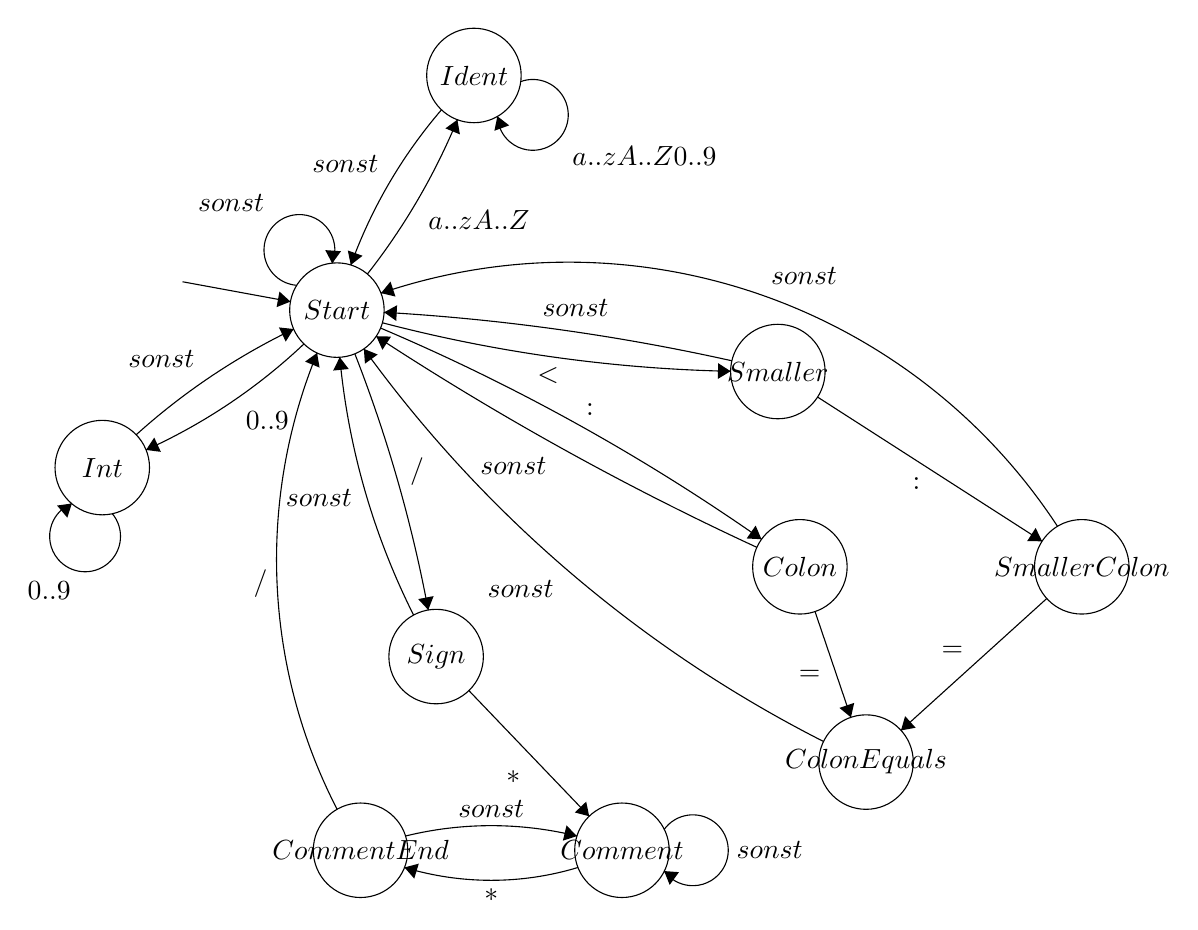
\begin{tikzpicture}[scale=0.2]
\tikzstyle{every node}+=[inner sep=0pt]
\draw [black] (16.7,-16) circle (3);
\draw (16.7,-16) node {$Start$};
\draw [black] (25.4,-1.1) circle (3);
\draw (25.4,-1.1) node {$Ident$};
\draw [black] (1.8,-26) circle (3);
\draw (1.8,-26) node {$Int$};
\draw [black] (44.7,-19.9) circle (3);
\draw (44.7,-19.9) node {$Smaller$};
\draw [black] (46.1,-32.3) circle (3);
\draw (46.1,-32.3) node {$Colon$};
\draw [black] (23,-38) circle (3);
\draw (23,-38) node {$Sign$};
\draw [black] (34.8,-50.3) circle (3);
\draw (34.8,-50.3) node {$Comment$};
\draw [black] (64,-32.3) circle (3);
\draw (64,-32.3) node {$SmallerColon$};
\draw [black] (50.3,-44.7) circle (3);
\draw (50.3,-44.7) node {$ColonEquals$};
\draw [black] (18.2,-50.3) circle (3);
\draw (18.2,-50.3) node {$CommentEnd$};
\draw [black] (14.16,-14.426) arc (265.94323:-22.05677:2.25);
\draw (9.98,-9.77) node [above] {$sonst$};
\fill [black] (16.4,-13.03) -- (16.96,-12.26) -- (15.96,-12.19);
\draw [black] (6.9,-14.2) -- (13.75,-15.46);
\fill [black] (13.75,-15.46) -- (13.05,-14.82) -- (12.87,-15.81);
\draw [black] (24.355,-3.911) arc (-22.45479:-38.10589:41.659);
\fill [black] (24.35,-3.91) -- (23.59,-4.46) -- (24.51,-4.84);
\draw (22.48,-10.25) node [right] {$a..zA..Z$};
\draw [black] (28.363,-1.491) arc (110.20708:-177.79292:2.25);
\draw (31.62,-6.19) node [right] {$a..zA..Z0..9$};
\fill [black] (26.89,-3.69) -- (26.7,-4.61) -- (27.64,-4.27);
\draw [black] (14.607,-18.148) arc (-46.6021:-65.66354:36.463);
\fill [black] (4.58,-24.88) -- (5.52,-25) -- (5.1,-24.09);
\draw (12.28,-22.43) node [below] {$0..9$};
\draw [black] (2.433,-28.92) arc (39.96376:-248.03624:2.25);
\draw (-1.57,-33.22) node [below] {$0..9$};
\fill [black] (-0.13,-28.28) -- (-1.07,-28.41) -- (-0.42,-29.18);
\draw [black] (3.955,-23.914) arc (132.03381:115.70055:42.381);
\fill [black] (13.95,-17.2) -- (13.02,-17.1) -- (13.45,-18);
\draw (5.56,-19.7) node [above] {$sonst$};
\draw [black] (17.584,-13.135) arc (160.12576:139.31356:31.593);
\fill [black] (17.58,-13.13) -- (18.33,-12.55) -- (17.39,-12.21);
\draw (19.36,-6.7) node [left] {$sonst$};
\draw [black] (41.7,-19.885) arc (-91.19157:-104.66736:95.135);
\fill [black] (41.7,-19.88) -- (40.91,-19.37) -- (40.89,-20.37);
\draw (30.11,-19.62) node [below] {$<$};
\draw [black] (19.475,-17.141) arc (66.99673:54.99339:132.256);
\fill [black] (43.66,-30.55) -- (43.29,-29.68) -- (42.72,-30.5);
\draw (32.77,-22.71) node [above] {$:$};
\draw [black] (17.839,-18.775) arc (21.36327:10.5963:90.178);
\fill [black] (22.5,-35.04) -- (22.84,-34.16) -- (21.86,-34.35);
\draw (21.32,-26.23) node [right] {$/$};
\draw [black] (25.08,-40.16) -- (32.72,-48.14);
\fill [black] (32.72,-48.14) -- (32.53,-47.21) -- (31.81,-47.9);
\draw (28.37,-45.62) node [left] {$*$};
\draw [black] (21.568,-35.364) arc (-153.35121:-174.68921:45.989);
\fill [black] (16.88,-18.99) -- (16.46,-19.84) -- (17.45,-19.74);
\draw (17.69,-27.96) node [left] {$sonst$};
\draw [black] (47.22,-21.52) -- (61.48,-30.68);
\fill [black] (61.48,-30.68) -- (61.07,-29.83) -- (60.53,-30.67);
\draw (53.5,-26.6) node [below] {$:$};
\draw [black] (19.697,-16.14) arc (86.69443:77.44664:138.285);
\fill [black] (19.7,-16.14) -- (20.47,-16.69) -- (20.52,-15.69);
\draw (31.85,-16.44) node [above] {$sonst$};
\draw [black] (47.06,-35.14) -- (49.34,-41.86);
\fill [black] (49.34,-41.86) -- (49.55,-40.94) -- (48.61,-41.26);
\draw (47.44,-39.22) node [left] {$=$};
\draw [black] (43.367,-31.064) arc (-114.79715:-123.21273:188.325);
\fill [black] (19.2,-17.66) -- (19.59,-18.52) -- (20.14,-17.68);
\draw (27.9,-25.31) node [below] {$sonst$};
\draw [black] (37.48,-48.977) arc (144:-144:2.25);
\draw (42.05,-50.3) node [right] {$sonst$};
\fill [black] (37.48,-51.62) -- (37.83,-52.5) -- (38.42,-51.69);
\draw [black] (32.009,-51.392) arc (-73.14481:-106.85519:19.001);
\fill [black] (20.99,-51.39) -- (21.61,-52.1) -- (21.9,-51.15);
\draw (26.5,-52.71) node [below] {$*$};
\draw [black] (21.058,-49.395) arc (103.80179:76.19821:22.812);
\fill [black] (31.94,-49.4) -- (31.28,-48.72) -- (31.05,-49.69);
\draw (26.5,-48.24) node [above] {$sonst$};
\draw [black] (16.712,-47.696) arc (-152.7312:-202.2607:34.615);
\fill [black] (15.44,-18.72) -- (14.68,-19.27) -- (15.6,-19.65);
\draw (12.33,-33.37) node [left] {$/$};
\draw [black] (61.78,-34.31) -- (52.52,-42.69);
\fill [black] (52.52,-42.69) -- (53.45,-42.52) -- (52.78,-41.78);
\draw (55.79,-38.01) node [above] {$=$};
\draw [black] (19.499,-14.923) arc (108.72765:33.24353:37.117);
\fill [black] (19.5,-14.92) -- (20.42,-15.14) -- (20.1,-14.19);
\draw (46.36,-14.38) node [above] {$sonst$};
\draw [black] (47.6,-43.392) arc (-116.89514:-144.11056:81.574);
\fill [black] (18.41,-18.46) -- (18.48,-19.4) -- (19.29,-18.82);
\draw (28.36,-33.16) node [below] {$sonst$};
\end{tikzpicture}
\end{center}

\chapter{Parsing}

Der Parser ist dafür zuständig die Token vom Scanner entgegen zu nehmen um dann daraus einen Syntaxbaum generieren zu können. Dabei überprüft der Parser syntaktische Korrektheit des Programms und gibt Fehlermeldungen aus falls er einen Syntaxfehler findet. Der Parser kann keine semantischen Fehler im Programm finden (z.B. die Zuweisung eines Integers an eine Variable, die ein Array referenziert), dies übernimmt der Typechecker, der aufgerufen wird sobald die Parsephase erfolgreich abgeschlossen wurde.

\section{Funktionsweise}
Der Parser ist ein \href{http://en.wikipedia.org/wiki/Recursive_descent_parser}{recursive-descent-parser} und parst folgende Grammatik:

\begin{verbatim}
PROG       ::= DECLS STATEMENTS
DECLS      ::= DECL ; DECLS | eps
DECL       ::= int ARRAY identifier
ARRAY      ::= [ integer ] | eps
STATEMENTS ::= STATEMENT ; STATEMENTS | eps
STATEMENT  ::= identifier INDEX := EXP
             | write ( EXP )
             | read ( identifier INDEX )
             | {STATEMENTS}
             | if ( EXP ) STATEMENT else STATEMENT
             | while ( EXP ) STATEMENT
EXP        ::= EXP2 OP_EXP
EXP2       ::= ( EXP ) | identifier INDEX | integer | - EXP2 | ! EXP2
INDEX      ::= [ EXP ] | eps
OP_EXP     ::= OP EXP | eps
OP         ::= + | - | * | / | < | > | = | <:> | &

eps = epsilon symbol
\end{verbatim}

Die obige Grammatik ist bereits eine \href{http://en.wikipedia.org/wiki/Parsing_expression_grammar}{parsing-expression-grammar} (PEG), d.h. Linksrekursion und Mehrdeutigkeiten wurden bereits aufgelöst. Der Parser parst also exakt diese Grammatik und wandelt sie in einen Syntaxbaum um, der exakt der PEG entspricht. Der Parser macht einen Lookup auf das nächste Token bevor er eine Rekursionsstufe tiefer geht, was allerdings nur passiert wenn er ein validen Token findet. Im Falle eines invaliden Tokens wird eine Fehlermeldung ausgegeben, die anzeigt welche Token erwartet und welches gefunden wurde.

Da der Parser die PEG exakt parst, wächst der Stack sehr schnell - bei auftretenden Überläufen im Parser muss der Stack also erhöht werden. Es ist möglich, die Grammatik so zu transformieren, dass der Stack nicht so stark wächst, dies wurde allerdings nicht umgesetzt. Der commit \texttt{050b035c5f717f460ae840574dbe0e8169cba916} enthält ein Beispiel, das zeigt, wie man den Stack in C++ erhöht.

\section{Parsebaum}
Da der Parsebaum die PEG exakt repräsentiert, besitzt er genau so viele unterschiedliche Knotentypen wie es Nichtterminale in der PEG gibt. Die Implementierung stellt aber nur einen Typ names \texttt{Node} bereit, der eine Methode namens \texttt{tpe} bereitstellt, über die der repräsentierte Typ herausgefunden werden kann. Der \texttt{Node} Typ besitzt weitere Methoden, über die man an dessen Inhalt herankommt. All diese Methoden sind abhängig vom repräsentierten Typ, wird versucht auf einen Inhalt zuzugreifen, der nicht repräsentiert wird so wird ein Laufzeitfehler ausgelöst. Ein Beispiel:

\begin{verbatim}
switch (node->tpe()) {
  case Nodes::Prog:
    node->decls(); // ok
    node->stmts(); // ok
    node->exp(); // Laufzeitfehler
    break;
  case ... // restliche Typen
}
\end{verbatim}

Die Namen der Methoden entsprechen in den meisten Fällen den Namen der Nichtterminale in der PEG, welcher Typ welche Operationen unterstützt steht in den Dokumentationskommentaren von \texttt{Node}.

Der Baum kann sehr einfach traversiert werden, die Vorgehensweise im Allgemeinen:

\begin{verbatim}
void traverse(Nodes::Node *node) {
  switch (node->tpe()) {
    case Nodes::Prog:
      traverse(node->decls());
      traverse(node->stmts());
      // behandle decls() und stmts() falls notwendig
      break;
    case ... // restliche Typen
  }
}
\end{verbatim}

Die Tests zu der Parserphase lassen sich im Verzeichnis \texttt{tests/parser} finden.

\chapter{Typechecking}

Beim Typechecking wird überprüft, ob die drei existierenden Typen \texttt{Int}, \texttt{IntArray} und \texttt{NoType} korrekt benutzt wurden und ob referenzierte Variablenbezeichner existieren und ob Operationen auf einem Typ definiert sind. Eine Fehlermeldung wird ausgegeben wenn ein Fehler gefunden wurde. Die Typüberprüfung wurde durch einen einfachen Traverser realisiert, der Baum muss nicht mehrere Male durchlaufen werden, da der erste Durchlauf alle möglichen Fehlermöglichkeiten bereits vollständig auflösen kann. Die gefundenen Typinformationen werden in dem, zum Variablenbezeichner zugehörigen \texttt{Symbol} abgelegt, das über den Baum referenziert werden kann.

Die Tests zu der Typisierungsphase lassen sich im Verzeichnis \texttt{tests/typer} finden.

\chapter{Codegenerierung}

Bei der Codegenerierung müssen keine Fehler im Syntaxbaum gesucht werden, alle möglichen Fehlerquellen wurden bereits aufgelöst. Die Codegenerierung funktioniert sehr einfach. Es ist wieder ein Traverser, der für jeden Knotentyp den zugehören Bytecode für die virtuelle Maschine ausspuckt. Die einzige Schwierigkeit liegt in der Generierung des Codes für die Operationen \texttt{> (größer)} und \texttt{<:> (ungleich)}, da diese von der virtuellen Maschine nicht unterstützt werden. Sie müssen durch Äquivalenzumformungen mit Hilfe von anderen Operationen repräsentiert werden.

Die Tests zu der Codegenerierungsphase lassen sich im Verzeichnis \texttt{tests/codegen} finden.

\end{document}
